\documentclass[11pt]{article}
\usepackage{mathunal-base}
\mathunalfuente{serif}

\renewcommand{\examtitulo}{Segundo Examen Parcial de Cálculo en Varias Variables}
\renewcommand{\examfecha}{12 de Mayo de 2014}

\begin{document}

\examheader

\vspace{4pt}
\noindent
\begin{minipage}[t]{0.62\linewidth}
Nombre \dotfill

\vspace{4pt}
Profesor \dotfill
\end{minipage}%
\hfill
\begin{minipage}[t]{0.32\linewidth}
Doc. Identidad \dotfill

\vspace{4pt}
Grupo \dotfill
\end{minipage}

\vspace{6pt}
\noindent\textbf{Instrucciones.} El examen tiene una duración de 1 hora y 40 minutos. \textbf{No se admiten preguntas durante el examen.} No está permitido el uso de calculadora, ni teléfonos móviles, ni cualquier otro tipo de aparato electrónico. Cualquier intento de fraude será sancionado con anulación del examen. En los puntos 2., 3. y 4. justifique sus respuestas.

\vspace{10pt}
\begin{enumerate}
\item{} (36\%) En los numerales (i)-(iv) escoja sólo una de las cinco opciones que se presentan. En el numeral (v) asocie la integral dada con su correspondiente gráfica. No se requiere que justifique sus respuestas.

\begin{enumerate}
\item{} (7\%) Sean $f(x,y)=x^2+y^2-xy+6x$ y $E=\{(x,y): y^2+x^2\leq 8\}$. De acuerdo al método de los multiplicadores de Lagrange, el sistema que se debe resolver para hallar los extremos de $f$ sobre la frontera de $E$ es:

\vspace{4pt}
\noindent
\begin{minipage}[t]{0.46\linewidth}
$a)\ \left\{\begin{aligned}2x-y+6&=2\lambda y\\ 2y-x&=2\lambda x\\ x^2+y^2&=8\end{aligned}\right.$
\end{minipage}%
\begin{minipage}[t]{0.5\linewidth}
$b)\ \left\{\begin{aligned}2x-y&=2\lambda x\\ 2y-x+6&=2\lambda y\\ x^2+y^2-8&=0\end{aligned}\right.$
\end{minipage}

\vspace{6pt}
\noindent
\begin{minipage}[t]{0.46\linewidth}
$c)\ \left\{\begin{aligned}2x-y+6&=2\lambda y\\ 2y-x&=2\lambda x\\ x^2+y^2&=8\lambda\end{aligned}\right.$
\end{minipage}%
\begin{minipage}[t]{0.5\linewidth}
$d)\ \left\{\begin{aligned}2x-y+6&=2\lambda x\\ 2y-x&=2\lambda y\\ x^2+y^2-8&=0\end{aligned}\right.$
\end{minipage}

\vspace{4pt}
\noindent $e)$ Ninguna de las anteriores.

\item{} (7\%) Sea $W$ el sólido en el primer octante acotado por la superficie $z=4-x^2-y^2$ y los planos $x=0$, $y=0$ y $z=0$. La integral que calcula el volumen de $W$ es:

\vspace{4pt}
\noindent $a)\ \int_0^{2\pi}\int_0^2\int_0^{4-r^2} r\,dz\,dr\,d\theta$.

\noindent $b)\ \int_0^{\pi/2}\int_0^2\int_0^{4-r^2} r\,dz\,dr\,d\theta$.

\noindent $c)\ \int_0^{\pi}\int_0^2\int_0^{4-r^2} r\,dz\,dr\,d\theta$.

\noindent $d)\ \int_0^{\pi/2}\int_0^4\int_0^{4-r} r\,dz\,dr\,d\theta$.

\noindent $e)$ Ninguna de las anteriores.

\item{} (7\%) Sean $B=\{(x,y)\in\mathbb{R}^2: 0\leq y\leq x^4\ \text{y}\ 0\leq x\leq 1\}$ y $f(x,y)=e^{x^2+y^2}$. Se sabe que el valor mínimo absoluto de $f$ en $B$ es $1$ y que el valor máximo absoluto de $f$ en $B$ es $e^2$. Entonces el valor de $\iint_B e^{x^2+y^2}\,dA$ se encuentra entre:

\vspace{4pt}
\noindent $a)$ $1$ y $e^2$. \hspace{1cm} $b)$ $1/5$ y $e^2/5$. \hspace{1cm} $c)$ $3/5$ y $3e^2/5$,

\noindent $d)$ $4/5$ y $4e^2/5$ \hspace{1cm} $e)$ Ninguna de las anteriores.

\item{} (7\%) Sea $E$ el sólido en el primer octante limitado por el cilindro parabólico $z=1-x^2$ y por los planos $z=0$, $y=0$, $x=0$ y $y=4-x$. La siguiente integral \textbf{NO} calcula el volumen de $E$:

\vspace{4pt}
\noindent $a)\ \int_0^1\int_0^{4-x}\int_0^{1-x^2}dz\,dy\,dx.$

\noindent $b)\ \int_0^1\int_0^{1-x^2}\int_0^{4-x}dy\,dz\,dx.$

\noindent $c)\ \int_0^1\int_0^{4-y}\int_0^{1-x^2}dz\,dx\,dy.$

\noindent $d)\ \int_0^1\int_0^{\sqrt{1-z}}\int_0^{4-x}dy\,dx\,dz.$

\noindent $e)$ Ninguna de las anteriores. Es decir, todas las anteriores calculan el volumen de $E$.

\item{} (8\%) Asocie cada región con la integral dada

\vspace{6pt}
\noindent
\begin{minipage}[t]{0.4\linewidth}
\begin{tabular}{|l|c|}
\hline
\textbf{Integral} & \textbf{Gráfica} \\ \hline
$\int_0^1\int_0^{x/2} f(x,y)\,dy\,dx$ & \\ \hline
$\int_0^1\int_0^{y} f(x,y)\,dx\,dy$ & \\ \hline
$\int_0^1\int_{x/2}^{x} f(x,y)\,dy\,dx$ & \\ \hline
$\int_0^1\int_{y/2}^{1} f(x,y)\,dx\,dy$ & \\ \hline
\end{tabular}
\end{minipage}%
\hfill
\begin{minipage}[t]{0.58\linewidth}
\begin{center}
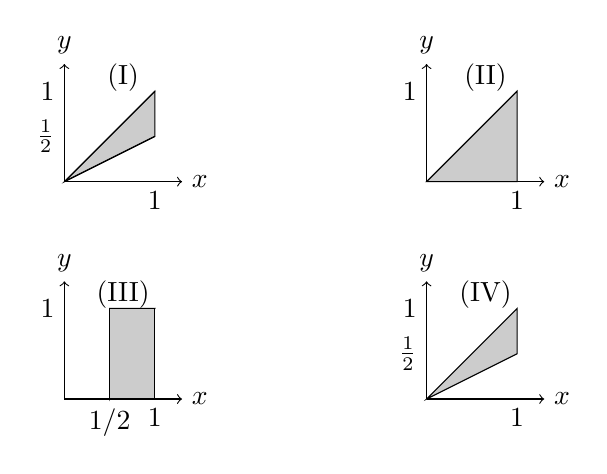
\begin{tikzpicture}[scale=1.15]
\begin{scope}
\draw[->] (0,0) -- (1.3,0) node[right]{$x$};
\draw[->] (0,0) -- (0,1.3) node[above]{$y$};
\draw[fill=gray!40] (0,0) -- (1,1) -- (1,0.5) -- cycle;
\draw (0,0) -- (1,1);
\draw (0,0) -- (1,0.5);
\node at (0.65,1.15) {(I)};
\node[left] at (0,1) {1};
\node[left] at (0,0.5) {$\frac{1}{2}$};
\node[below] at (1,0) {1};
\end{scope}
\begin{scope}[xshift=4cm]
\draw[->] (0,0) -- (1.3,0) node[right]{$x$};
\draw[->] (0,0) -- (0,1.3) node[above]{$y$};
\draw[fill=gray!40] (0,0) -- (1,1) -- (1,0) -- cycle;
\node at (0.65,1.15) {(II)};
\node[left] at (0,1) {1};
\node[below] at (1,0) {1};
\end{scope}
\begin{scope}[yshift=-2.4cm]
\draw[->] (0,0) -- (1.3,0) node[right]{$x$};
\draw[->] (0,0) -- (0,1.3) node[above]{$y$};
\draw[fill=gray!40] (0.5,0) -- (1,1) -- (0.5,1) -- cycle;
\draw[fill=gray!40] (0.5,0) -- (1,0) -- (1,1) -- (0.5,1) -- cycle;
\node at (0.65,1.15) {(III)};
\node[left] at (0,1) {1};
\node[below] at (0.5,0) {1/2};
\node[below] at (1,0) {1};
\end{scope}
\begin{scope}[xshift=4cm,yshift=-2.4cm]
\draw[->] (0,0) -- (1.3,0) node[right]{$x$};
\draw[->] (0,0) -- (0,1.3) node[above]{$y$};
\draw[fill=gray!40] (0,0) -- (1,1) -- (1,0.5) -- cycle;
\node at (0.65,1.15) {(IV)};
\node[left] at (0,1) {1};
\node[left] at (0,0.5) {$\frac{1}{2}$};
\node[below] at (1,0) {1};
\end{scope}
\end{tikzpicture}
\end{center}
\end{minipage}
\end{enumerate}

\newpage
\item{} (15\%) Sea $W$ el sólido que está dentro de la superficie $x^2+y^2+z^2=2z$ y fuera de la superficie $x^2+y^2+z^2=z$. Suponga que en todo punto de $W$ la densidad es directamente proporcional a su distancia al origen. Dibuje la región $W$ y \textbf{plantee} (sin resolver) la integral que calcula su masa en coordenadas esféricas.

\vspace{6cm}

\item{} (24\%) Sea $D\subseteq\mathbb{R}^2$ la región del primer cuadrante acotada por las curvas $y=0$, $y=1$, $x=\sqrt[3]{y}$ y $x=1$. Dibuje la región $D$ y calcule
\[
\iint_D \sqrt{1+x^4}\,dA.
\]

\vspace{7cm}

\item{} (25\%) Sea $D$ la región del plano acotada por las rectas $y=1-x$, $y=2-x$, $y=x-1$ y $y=x+1$. Calcule
\[
\iint_D \frac{\cos(y-x)}{y+x}\,dA.
\]
\noindent Dibuje claramente la región de integración de toda integral que escriba.

\vspace{7cm}
\end{enumerate}

\examfooter
\end{document}
